\documentclass[12pt, a4paper, abstract, parskip]{scrartcl}
\def\datum{\today}
\author{Tobias Raabe}
\title{Identification Strategies of Software Patents}

\usepackage[english]{babel}
\usepackage[utf8]{inputenc}
\usepackage[T1]{fontenc}
\usepackage{lmodern}
\usepackage{booktabs}
\newcommand{\ra}[1]{\renewcommand{\arraystretch}{#1}}
\usepackage{amsmath, amssymb, amsthm}
\usepackage{nameref}
\usepackage{graphicx}
\usepackage[space]{grffile}
\usepackage[hidelinks, hyperfootnotes=false]{hyperref}

\usepackage{geometry} % Anpassung der Seite
\geometry{left=30mm,right=20mm,top=20mm,bottom=20mm}
\usepackage{setspace} % Defines Line spacing
\onehalfspacing
\usepackage[section]{placeins}

\usepackage{epigraph}
% \epigraphsize{\small}% Default
\setlength\epigraphwidth{14cm}
\setlength\epigraphrule{0pt}
\usepackage{etoolbox}
\makeatletter
\patchcmd{\epigraph}{\@epitext{#1}}{\itshape\@epitext{#1}}{}{}
\makeatother

\usepackage[backend=biber, natbib=true, bibencoding=utf8, safeinputenc=true,
bibstyle=authoryear, citestyle=authoryear-comp, maxcitenames=2, mincitenames=1,
uniquelist=false, useprefix=true, maxbibnames=99, minbibnames=99, backref=true,
backrefstyle=three, doi=true, isbn=false, sortcites=false, dashed=false,
]{biblatex}
\addbibresource{references.bib}

\theoremstyle{definition}
\newtheorem{definition}{Definition}[subsection]

\begin{document}

\pagenumbering{roman}

\newpage
\vspace*{2cm}
\begin{center}
\thispagestyle{empty}
\rule{14cm}{1pt}\\[1cm]
{\huge Identification Strategies of Software Patents}\\[1cm]
\rule{12cm}{1pt}\\[3cm]
\textbf{\large Bachelorarbeit zur Erlangung des Grades}\\[4pt]
\textbf{\large Bachelor of Science (B.Sc.)}\\[1cm]
{\large im Studiengang Volkswirtschaftlehre}\\[1cm]
\textbf{\large an der Rheinischen Friedrich-Wilhelms-Universität zu Bonn}\\[4pt]
{\large JProf. Michael Böhm}\\[4cm]
\begin{tabular}{rl}
\hline
Autor: & Tobias Raabe\\
Studiengang: & Volkswirtschaftslehre\\
Matrikelnummer: & 2573626\\
E-Mail: & tobiasraabe@uni-bonn.de\\
Vorgelegt: & September 2015\\
\hline
\end{tabular}
\end{center}
\newpage

\renewcommand*{\abstractname}{\large Abstract}
\begin{abstract}
    This Bachelor's Thesis is about the identification of software patents,
    which build a substantial group among patents without a specific class id
    in the USPTO categorization system. Knowing the number of not only software
    patents, but also other distinct patent groups allows drawing conclusions
    of the relationship to economic developments such as increasing
    productivity or the rapid number of patent infringement cases due to patent
    trolls. The focus of this thesis is on identification strategies for
    patents, since they are not categorized as mentioned before. Firstly, an
    algorithmic approach of \citet{bessen2007empirical} is replicated which
    evaluates the type of document by a combination of keywords. Secondly,
    machine learning techniques are exploited which use the whole text as
    input. The advantages of this approach are discussed and further
    improvements are mentioned.
\end{abstract}

\newpage
\tableofcontents

\newpage

\pagenumbering{arabic}

\epigraph{"Begin at the beginning," the King said gravely, "and go on till you
come to the end: then stop."}{--- \textup{Lewis Carroll}, Alice in Wonderland}

\section{Introduction}
\label{sec:introduction}

This thesis is about software patents and different ways to classify them which
are called identification strategies. It can be separated in two parts. The
first part is about patents as an economically influential concept and the
first question is: What kind of data are patents? After that, the quality of
patents as an indicator is examined and applications are presented. The second
part is concerned with the identification of patents on a specific topic. As
subsequently shown, the solution to this task is not obvious since patent
databases are not structured to serve the research interest of economists. The
first approach is a replication of \citet{bessen2007empirical}, the main
inspiration for this thesis. After that, machine learning techniques are
explored as an alternative technique to identify patents.

% section introduction (end)


\section{Background and Data} % (fold)
\label{sec:background_and_data}

First of all, what is a patent? A patent is a property right which is granted
by a patent office, in this case the USPTO (United States Patent and Trademark
Office)\footnote{This thesis limits itself to the US patent system since it
dominates worldwide in magnitude and importance.}. The patent term which is the
duration of protection is nowadays 20 years from the filing date and was last
changed in 1994, where it were previously only 17 years. Patents have to be
distinguished from trademarks / servicemarks, which indicate the source of
goods and services, and from copyright, a protection of intellectual works in
art. Furthermore, the USPTO differentiates between utility patents, design
patents, and plant patents. This thesis concentrates on utility patents, which
are new and useful\footnote{Both terms are explained later.} devices and
methods or new and useful improvements of existing inventions. So, whenever the
term patent is used in this thesis utility patents are meant, if not otherwise
identified.

Patents can be beneficial for society. For example, the patent term ensures
inventors to have a monopoly for a period of time on the patent's invention and
to claim fees. The amount of investment in R\&D should rise, because the risk
is lowered. Furthermore, patents facilitate trading of technology, could be an
indicator for successful start-ups. Additionally, the disclosure of technical
details helps spreading knowledge. But patents can also provide several
disadvantages to society. One empirical observation is called patent thickets,
when big firms accumulate large stacks of patents to restrict the entry to
their industry or to extract rents from other firms. Another aspect of patent
rights is the risk of litigation, which has to be considered if one makes a
investment. Similar and undiscovered patents, also called submarine patents,
could potentially be the basis for injunction lawsuit, but the acquisition of
those or even the search for them could be costly. Then, the investment would
be riskier\footnote{see \citet{bessen2011generation}}.

Concerning the case of patent infringement, the plaintiff has to address
federal courts because the patent office has no jurisdiction. During the
examination process, the question whether the examined patent infringes any
existing and still protected patents is not answered. If a protection is
violated, the plaintiff can sue for injunction to discontinue the infringement
and / or sue for compensation.

The two main requirements for obtaining a patent are novelty and
non-obviousness and are applicated during the examination process. There are
two conditions for novelty: First, the invention must not have been available
to the public before the filing date of the invention and, second, it must not
have been mentioned in an issued patent, called prior art. When these criteria
are met, patent status can still be refused, in case the difference between the
invention and prior art is obvious for <<a person, having ordinary skill in the
area of technology related to the invention>>\footnote{see
\cite{uspto2014patents}}. One might think, that these two requirements set high
levels for patent status, but in 1980 for example 104,000 patents were applied
and 61,000 were granted, a ratio of circa 58\%. The ratio for different years
is 62\% in 1970, 54\% in 1990, 53\% in 2000, and 44\% in 2010\footnote{The
statistics are from URL \#1 in Table~\ref{tab:url}}. The ratios for the
European Patent Office for all patents from 2005 till 2014 vary from 23\% to
29\%\footnote{The patent filing statistics are from URL \#2 and the granting
statistics from URL \#3 in Table~\ref{tab:url}}. These number are only examples
and should not be interpreted as a trend in the US to a stricter granting
process. But, one can observe, the numbers are varying over the years and
countries, which is, according to \citet{griliches1990patent}, related to the
procedures and resources of patent offices and therefore also indicate the
quality of patents. Numbers on patents are also available for firms,
industries, and countries and allow to examine the relation of patents on the
economy in different contexts\footnote{\cite{hall2001nber} provide a rich and
already harmonized database on patents, citations, et cetera matched with data
from Compustat, data for all firms traded in the US. The dataset is called the
\textit{NBER U.S. Patent Citations Data File} and is available under URL \#4 in
Table~\ref{tab:url}}. This commonality measure of the previous mentioned data
is based on patent counts grouped by other variables to identify effects. But,
patent data is a much richer resource than that, because a patent also contains
links to similar patents and can cite scientific publications not forgetting
the patent's text with description and claims.

\citet{griliches1990patent} names two major problems to use patents in economic
analysis: First, patents are not like one another in terms of importance. Most
patents provide only small improvements on existing knowledge and therefore, an
aggregated measure containing simple patent counts is a biased measure for
technological progress. The second problem is classification, as the U.S.
Patent Classification System (USPC) contains more than 450 classes and circa
150,000 subclasses which are not restricted to certain classes\footnote{see
\citet{uspto2012}}. It is primarily based on technological and functional form.
\citeauthor{schmookler1966invention} states to that:

\epigraph{"A subclass dealing with the dispensing of liquids contains both a
patent for a water pistol and one for a holy water dispenser. Another subclass
relating to the dispensing of solids contains patents on both manure spreaders
and toothpaste tubes"}{--- \textup{\citeauthor{schmookler1966invention}},
Invention and economic growth (1966), p.20}

Still, some researchers tried to rehash the use of the existing classification
system by examining the concordance between their patents of interest and
different subclasses. If the similarity is big enough, the subclasses are used
in the inquiry. Another approach was done by \citeauthor{hall2001nber}, who
traced back to the origin of the patent, meaning the firm. Then, patents can be
assigned to industries based on the owner's business. This can be useful for
research on firm level; Nonetheless, it is highly impracticable for broader
contexts such as industry levels, because of the diversified nature of some
businesses and the spillover of knowledge into other fields than the owner's
business\footnote{see \cite{griliches1990patent}}.

Another issue is that the classification system changes over time and patents
are reclassified, which prevent longitudinal studies to make time consistent
results\footnote{see \citet{bessen2007empirical}}. Furthermore, applicants try
to influence the examination process, hoping that their patent falls into a
different class\footnote{see, \citet[p.21]{lerner2006new}}.

Once an understanding for the underlying data is established, one can focus on
the use of patent statistics to examine economical observations. Hence the
question bears <<What aspects of economic activity do patent statistics
actually capture?>> \citep[p. 296]{griliches1990patent}. Economists would
preferably measure the changes in economically relevant knowledge. This
progress can be seen as an output of investment in research, R\&D for example,
and other unknown variables. Following this idea, patents are one expression of
this technological progress, but also influenced by other variables like cost-
effectiveness or patent propensity. The variable economists are primarily
interested in is determined by progress, by other variables, and noise. This
model is a strong simplification of reality and needs a lot of assumptions. For
example, a decline in existing knowledge has to be modeled, R\&D is exogenous,
patents have no economical influence, reverse causality, et cetera. But the
main point of this model is that the correlation between R\&D as an input
factor and knowledge and also the correlation of patents, which can be seen as
an indicator for the success of knowledge creation, and knowledge is both
unobserved. Therefore, depending on the situation R\&D or patents could be a
better indicator to knowledge. Another idea is the correlation of R\&D as input
and patents as output among other influences can be seen as a lower bound of
knowledge creation.

Since patents and R\&D are important to progress, not only according to this
model, it is worth looking at the connection between both to access their
quality as an indicator. \cite{griliches1990patent} cites many important
research in this domain which will be shortly presented.

A cross-sectional study reveals a strong connection between R\&D and the number
of patents received on the level of firms and industries with an $R^2$ of 0.9,
strengthening the idea of patents as an indicator. The results for a within-
firms time series study are much weaker but still significant with an $R^2$ of
0.3. The changes in R\&D also occur almost simultaneously which is at first
surprising, but corresponds with the observation that patents are applied for
early in the development process. What might be puzzling is that regressing
patents on R\&D in time-series studies yields significantly lower coefficients
than on the cross-sectional level.

One important question regarding patents is, whether there are diminishing
returns to R\&D. Time-series studies found weak evidence that the ratio of
patents per R\&D investment is declining, which may indicate that research
opportunities are depleted, but these findings are highly depending on
functional form. Cross-sectionally one can observe that the patent per R\&D
ratio is much higher for small businesses, then declines rapidly and flattens
for large businesses. But the reason for that lies not in diminishing returns
to R\&D. First of all, the data is drawn from firms listed on NYSE and
therefore the small firms are the highly selective winner of a much bigger
sample, having extraordinary characteristics as much patents. Another reason is
that small businesses report less R\&D to appear more effective and valuable.
Also, their success relies more on patents than bigger businesses, which leads
to different propensity.

Another time-series study estimates elasticities between 0.3 and 0.6 for
regressing patents on R\&D. These results are robust to functional forms and
lagged variables. Since the authors expect measurement errors in R\&D, because
the reported value is not the same used for patentable inventions, the
coefficients could be downward biased. Therefore, they run the regression the
other way round, R\&D on patents, to estimate a lower bound for the
coefficient. The values are 0.1-0.2, an indication for increasing returns.
Hence, the hypothesis of diminishing returns is highly controversial.

R\&D and patents are highly depending on industries. For example, industries
with the highest absolute numbers of patents are drugs, plastics, computers,
instruments, communication equipment and industrial chemicals. The counterpart
are large R\&D industries like motor vehicles and aircraft. Apart from that,
the results are not clear and even an attempt to relate patent propensity to
the perceived effectiveness of patents in various industries could not clarify
the the view.

% section background_and_data (end)


\section{Empirical Research on Patents} % (fold)
\label{sec:empirical_research_on_patents}

So far, the thesis has explained why identification strategies are a useful
tool for economical research and the appropriability of patents as an indicator
for technological progress was discussed. Two scientific examinations are
presented, which used some form of identification strategy for patents. The
first is \citet{bessen2007empirical} and the second is \cite{graham2013smart}.

\subsection{Empirical Look at Software Patents} % (fold)
\label{sub:empirical_look_at_software_patents}

The underlying paper for this thesis was \cite{bessen2007empirical} and their
reason to establish an algorithmic approach to identify software patents was to
examine the reasons of a rapidly growing number of software patents. They
suspected certain firms known for strategic patenting to strongly influence
this development along with legal changes on the patentability of software
patents. From 1987 to 1996 the number of software patents rose by 16\%
annually, whereas production factors experienced significant lower increases
\footnote{R\&D: 4.4\% p.a., employment in computer programming related jobs:
7.1\% p.a., real business spending on own-account and outsourced programming:
7.4\% p.a.}. Simultaneously, general patent propensity went up by 2.1\% per
year.

Given the data on input factors, they used a model of a patent production
function to estimate the explained rise in software patents by the input
factors. Their results indicate that only a minor share of 5.3\% can be
attributed to capital, employment, et cetera, whereas the majority of 10.8\% is
captured by year dummies and is interpreted as software patent propensity.

They also find differences in software patent propensity among different
industries. When they first evaluated which firms obtain software patents, they
found out manufacturing firms\footnote{SIC 35: industrial machinery \&
equipment, SIC 36: electronic \& other electronic equipment, SIC 38:
instruments \& related products} and IBM account for 68\% of all software
patents, whereas software publishers and software firms\footnote{SIC 737:
software publishers and service, SIC 7372: software publishers} excluding IBM
acquire only 7\% of all software patents. They argue, that this distribution
hardly reflects software creation.

Returning to software patent propensity, \citeauthor{bessen2007empirical}
address the issue that software developers could be more productive. They find
a positive relationship, but it contributes only 0.5\%. Another objection is
that changes in copyright made software patenting relatively cheaper and
therefore causes the change in propensity, but this effect is also not
significant large.

% subsection empirical_look_at_software_patents (end)


\subsection{Of Smart Phone Wars and Software Patents} % (fold)
\label{sub:of_smart_phone_wars_and_software_patents}

The second study is \citet{graham2013smart} and focuses partly on the claim
that software patents have a lower quality than other patents. The assumption
was that the so-called <<smartphone patent wars>>, a business battle between
smartphone manufacturer and software developer, prominently Sony, Google, Apple
Inc., Samsung, Microsoft, Nokia, et cetera, suing and counter-suing each other
for patent infringement, were mainly driven by the uncertainty created by
software patents. The start of the wars might be allocated in 2009, when Nokia
sued Apple over ten patents in October\footnote{An article is available under
url \#5 in Table~\ref{tab:url}} and Apple counter-suing Nokia in December over
13 patents\footnote{An article is available under URL \#6 in
Table~\ref{tab:url}}.

The authors examined patents involved in high-profile litigation and found 21
patents which could be interpreted as software patents according to a patent
office examiner. Court rulings affirmed the patent status of 17 of them and
rejected four. The authors state that the 80\% approval rate by the Federal
courts is comparable to court rulings on other technology.

To expand the analysis, \citeauthor{graham2013smart} first defined software
patents as patents <<containing some element of either general purpose software
or software that is specific to some form of
hardware>>\citep[p.~75]{graham2013smart}. Then, patent office experts examined
all classes of the USPC and collected the classes and subclasses which were
likely to contain software patents. Patents in this classes are labeled
software patents and used to analyze the application process of patents for
differences.

First, they investigated the numbers of First Final Actions for software and
other patents. After an examiner at the patent office rejects a patent
application, the applicant can oppose the decision and deliver new arguments in
favor of the application. The examiner will re-investigate and will make a Final
Action. Among the First Final Actions that were rejections from 2003 to 2012
they find that annual as well as cumulative differences were significant and
indicate that software patents received more rejections than others.

Concerning the trend of decreasing rejections since 2009, the authors argue
that this finding might be due to better interaction between examiner and
applicant. The authors address the issue that these finding could also indicate
that the examination process for both patents is softer. But the results of
USPTO's internal quality assurance suggests that the rate of compliance with
patent law for both groups among 2007 and 2012 is not significantly different.
The results are obtained by randomly reviewing 29,000 patents. The rates of
allowances differ between 96.5\% for non-software patents and 96.8\% for
software patents. The rates of rejections are 93.5\% for non-software and
93.6\% for software.

Another internal check of the validity of rejection and allowances is from the
board of patent appeals. Since 2008 one can observe a higher affirmance rate
which is 8.2 percentage points higher than for non-software significant at the
5\% level. Furthermore, the decisions of the board of patent appeals can be
reviewed by the US Court of Appeals, which confirms rejections with a rate of
95\%.

The authors conclude that the claims of a less intensive examination of
software patents cannot be upheld, because rejections were confirmed at
multiple stages, namely two intern assessments and Federal Courts.

% subsection of_smart_phone_wars_and_software_patents (end)
% section empirical_research_on_patents (end)


\section{An Algorithmic Approach} % (fold)
\label{sub:an_algorithmic_approach}

The following two sections focus on the methodological approach of software
patent detection. The first approach explained in this section is a replication
of the algorithm used by \cite{bessen2007empirical}. After that, the algorithm
will be evaluated by using information retrieval techniques. In the following
section, machine learning techniques are exploited, which prove to be useful
tool in the field of Natural Language Processing (NLP).

But, before starting with the analysis, software patents have to be defined.
Since this thesis orients itself towards \cite{bessen2007empirical} it will
also share their definition of a software patent:

\epigraph{"Our concept of software patent involves a logic algorithm for
processing data that is implemented via stored instructions; that is, the logic
is not "hard-wired". These instructions could reside on a disk or other storage
medium or they could be stored in "firmware", that is, a read-only memory, as
is typical of embedded software. But we want to exclude inventions that do not
use software as part of the invention. For example, some patents reference off-
the-shelf software used to determine key parameters of the invention; such uses
do not make the patent a software patent."}{---
\textup{\citeauthor{bessen2007empirical}}, Empirical Look at Software Patents
(2007), p.7}

According to this definition, \citet[p.8]{bessen2007empirical} classified a
sample of 399 patents between the years 1996-98\footnote{Initially, the sample
comprised 400 patents, but the patent US5785646 was withdrawn (URL \#7 in
Table~\ref{tab:url}), which can happen because of several reasons (URL \#8 in
Table~\ref{tab:url}). For example, the issue fee is not paid}. This
sample\footnote{The sample was gratefully provided for me by Jim Bessen} serves
as a benchmark to evaluate the power of their algorithm and to justify further
inferences. They searched the USPTO's database for patent's texts and stored
occurrences of words, they believed to be important for the identification
process. They found out about these words by classifying a random sample of
patents. Finally, they built an algorithm\footnote{A pseudo code for this
algorithm is in the appendix (\ref{def:algo})}, which states that a patent is
or is not software related based on a boolean construction of word occurrences
and their position in the text.

But before turning to the results, one should think about which errors the
algorithm might make and what could be an appropriate metric to measure its
power.

\subsection{Excursion: Evaluation of Algorithms}

\begin{table}[tb]\caption{Confusion Matrix of \cite{bessen2007empirical}}\label{tab:confusion_algo_original}\centering\ra{1.3}
    \input{../../out/tables/tab-cf-replication-bh-with-crawled-text}
\end{table}

The evaluation starts with a confusion matrix
(Table~\ref{tab:confusion_algo_original}) of \citeauthor{bessen2007empirical}'s
algorithm, which tabulates labels and predictions. If the document is manually
classified as a software patent it is in the group of relevant documents.
Furthermore, a document is retrieved if the algorithm states that it is a
software patent. If one would intuitively design a measurement to evaluate the
algorithm, it would likely be accuracy. Accuracy sums up the correct classified
information, true-positives and true-negatives, divided by the total number of
information\footnote{All measures are explained in
Table~\ref{tab:definition_measure} following the terminology of
Table~\ref{tab:confusion_example}}. The Accuracy for the confusion matrix is:

\begin{align*}
\text{Accuracy} &= \frac{\text{true-positives} + \text{true-
negatives}}{\text{total number of information}} = \frac{42 + 337}{399} \approx
95\%
\end{align*}

But this measurement is not useful for this kind of skewed data. The amount of
classified software patents is about 13.5\%\footnote{$\text{Share of software
patents} = \frac{54}{399} \approx 13.5\%$} and an algorithm which would not
retrieve a single document would have a decent accuracy, but no substance. So,
a statistic is needed, which differentiates between types of errors and
controls for the skewness at the same time.

Therefore, \citeauthor{bessen2007empirical} introduce precision and
recall\footnote{They use different terms for the same concept. Recall is what
they refer to as power and $(1-\text{Accuracy})$ is precision. The terminology
in this thesis sticks to precision and recall, since these terms seem to be
more common in science (\citet[p.~155]{manning2008introduction},
\citet[p.~2]{powers2011evaluation}, \citet[p.~2]{fawcett2006introduction}) and
prevent ambiguities.}. Precision is defined as the true positive rate given the
information is retrieved and recall refers to the true positive rate given the
information is relevant\footnote{see Table~\ref{tab:definition_measure}}.
Considering Table~\ref{tab:confusion_algo_original} again, precision and recall
are calculated in this way:

\begin{align*}
\text{Precision} &= \frac{tp}{tp + fp} = \frac{42}{42 + 8} \approx 84\% \\
\text{Recall} &= \frac{tp}{tp + fn} = \frac{42}{42 + 12} \approx 78\%
\end{align*}

Having two numbers for different errors can be a great advantage. For example,
a computer scientist is programming a spam detector for an e-mail program. The
worst error the detector can make is to label common e-mails as spam because
spam is dropped in a specific folder and is likely to be never seen by the
user. Because of that, the programmer is mainly concerned about precision. In
contrast, searches on hard disks are allowed to deliver results which are not
important, but the results must contain the desired item. Hence the focus is on
recall. Recognizing the fact that one can always achieve a recall of 1 if all
information is labeled software by the classifier, precision and recall form a
trade-off in errors. Recall is normally non-decreasing in the number of
retrieved information, but precision is decreasing\footnote{see
\citet[p.~156]{manning2008introduction}}.

Returning to the problem of software patent detection, both errors, precision
and recall, are crucial for the analysis. Still, the metric does not take into
account the number of true negatives. Considering the confusion matrix in
Table~\ref{tab:confusion_algo_original}, precision and recall are not changed
if the number of true-negatives varies. Nevertheless, one would intuitively
favor the second model. In addition to that, a better metric should yield an
overall value so that one can see whether the trade-off is exploited at best.
This is especially useful for machine learning during the process of parameter
tuning. There are a number of different measures for example the F measure,
which is the harmonic mean of precision and recall, ROC analysis, et
cetera\footnote{see \cite{manning2008introduction},
\cite{powers2011evaluation}, \cite{fawcett2006introduction}}. The metric used
in this analysis is $\kappa$, which was first mentioned in
\cite{cohen1960coefficient} and the original intent was to measure the
agreement or disagreement of two or more people observing the same phenomenon.
If one rater is then replaced by an objective measure, one can access the
rater's agreement with reality. In machine learning it can be used to measure
agreement and disagreement of a classifier with reality and to compare
different tuned versions of the same classification model, because each is seen
as an individual classifier.. $\kappa$\footnote{Definitions can be found in
Table~\ref{tab:definition_measure}} is based on accuracy, but controls for the
fact that correct classification could be a result of coincidental concordance
between the classifier's output and the label-generation process. The main
reason to use $\kappa$ over F measure and ROC was it appeared to be more
connected to intuitively correct results. The formula for $\kappa$ is:

\begin{align*}
\kappa &= \frac{\text{Accuracy} - \text{Expected Accuracy}}{1- \text{Expected Accuracy}}
\end{align*}

Accuracy is the same measure as mentioned above. Expected Accuracy is the
combined probability of information being retrieved and relevant plus the
probability of information being no t retrieved and not relevant.

\begin{align*}
\text{Expected Accuracy} &= p(\text{retrieved})\cdot p(\text{relevant}) + p(\text{not retrieved}) \cdot p(\text{not retrieved})\\
&= \frac{42 + 8}{399}\cdot\frac{42 + 12}{399} + \frac{12 + 337}{399}\cdot\frac{8+337}{399}\\
&\approx 78\%
\end{align*}

Now, it possible to calculate the $\kappa$ statistic for the original results,
when the Accuracy of the algorithm is:

\begin{align*}
\kappa &= \frac{\text{Accuracy} - \text{Expected Accuracy}}{1- \text{Expected Accuracy}}\\
&= \frac{0.95 - 0.78}{1-0.78} \approx 77\%
\end{align*}

But how does one interpret different $\kappa$ values?
\citet[p.~8]{landis1977measurement} propose an arbitrary division of $\kappa$
values from 0-0.20 as slight, 0.21-0.40 as fair, 0.41-0.60 as moderate,
0.61-0.80 as substantial, and 0.81-1 as almost perfect. Nonetheless, an
evaluation should never exclude the confusion matrix for a more detailed view
on the errors made by the algorithm.

\subsection{Discussion of Results} % (fold)
\label{ssub:discussion_of_results}

The results of \citet{bessen2007empirical} in
Table~\ref{tab:confusion_algo_original} and of the replication in
Table~\ref{tab:confusion_algo_rep} are very strong considering the simplicity
of the algorithm and the sparse amount of information processed. The authors
argue that strict rules of the USPTO incentivize patent drafters to use exact
language. Otherwise, their product is not covered by the patent or the patent
may not be granted\footnote{see \citet[pp.~7-9]{bessen2007empirical}}. Another
concern for heuristic approaches might be human overfitting: If the person who
is given the task of labeling the data knows anything about the type of
algorithm that will be built to classify the data later on, it is not ensured,
that the labeling process is not influenced by that.

Another issue is the test sample comprises only patents from 1996-98.
Naturally, one would assume that language evolves over time and maybe even in a
rigid patent system this could lead to different results for the algorithm for
different periods of time. This is a serious concern for this thesis because
the algorithm is applied on patents from 1976 to 2015 without testing on a
sample which is bigger and balanced among the years.

\begin{table}[tb]\caption{Confusion Matrix of the replication}\label{tab:confusion_algo_rep}\centering\ra{1.3}
    \input{../../out/tables/tab-cf-replication-bh-with-crawled-text}
\end{table}

The confusion matrices of both, the original in
Table~\ref{tab:confusion_algo_original} and the replication in
Table~\ref{tab:confusion_algo_rep}, have only slight differences. They might be
explained by differences in the patent's text recognition, excluding headings,
claims, et cetera.

The precision, recall, and kappa statistics of both, the original and the
replication, can be seen in Table~\ref{tab:eval_algo_original} and
Table~\ref{tab:eval_algo_rep}.

\begin{figure}[tb]
	\centering
	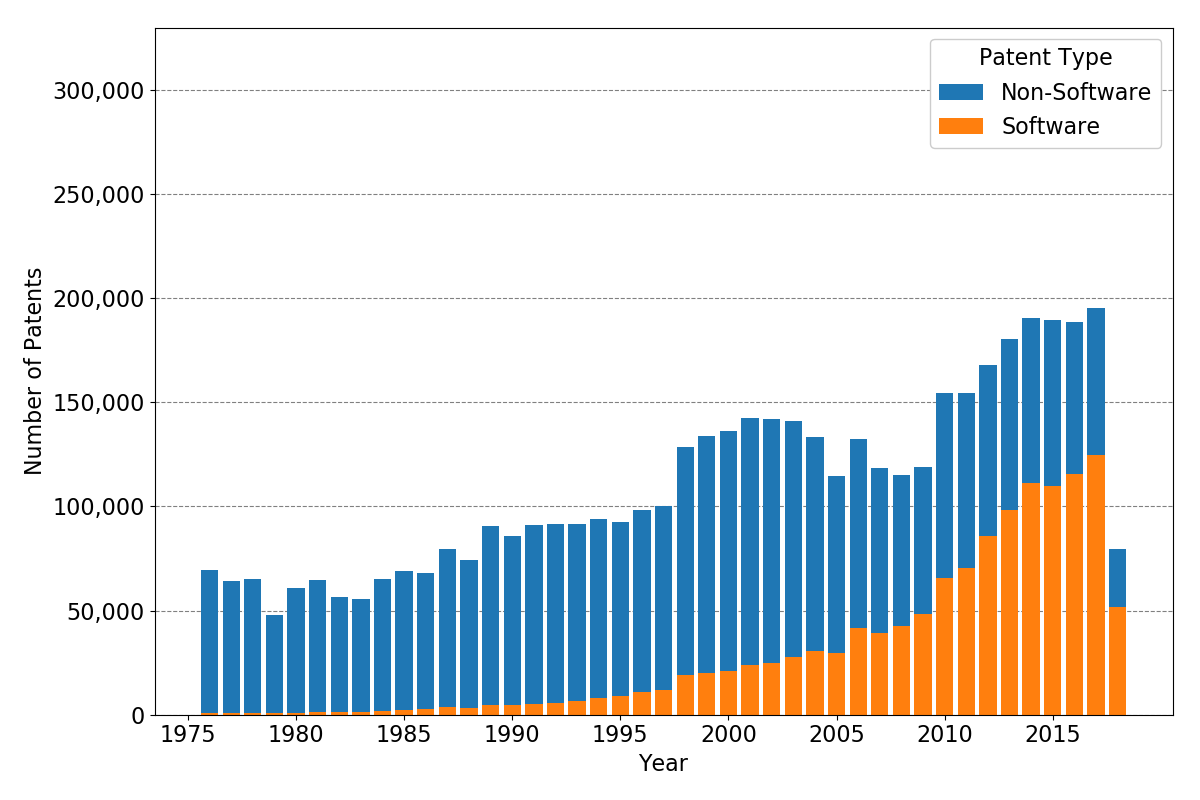
\includegraphics[width=0.7\textwidth]{../../out/figures/fig-patents-distribution-vs}
	\caption{Number of Software Patents}
	\label{fig:softpat}
\end{figure}

\begin{figure}[tb]
	\centering
	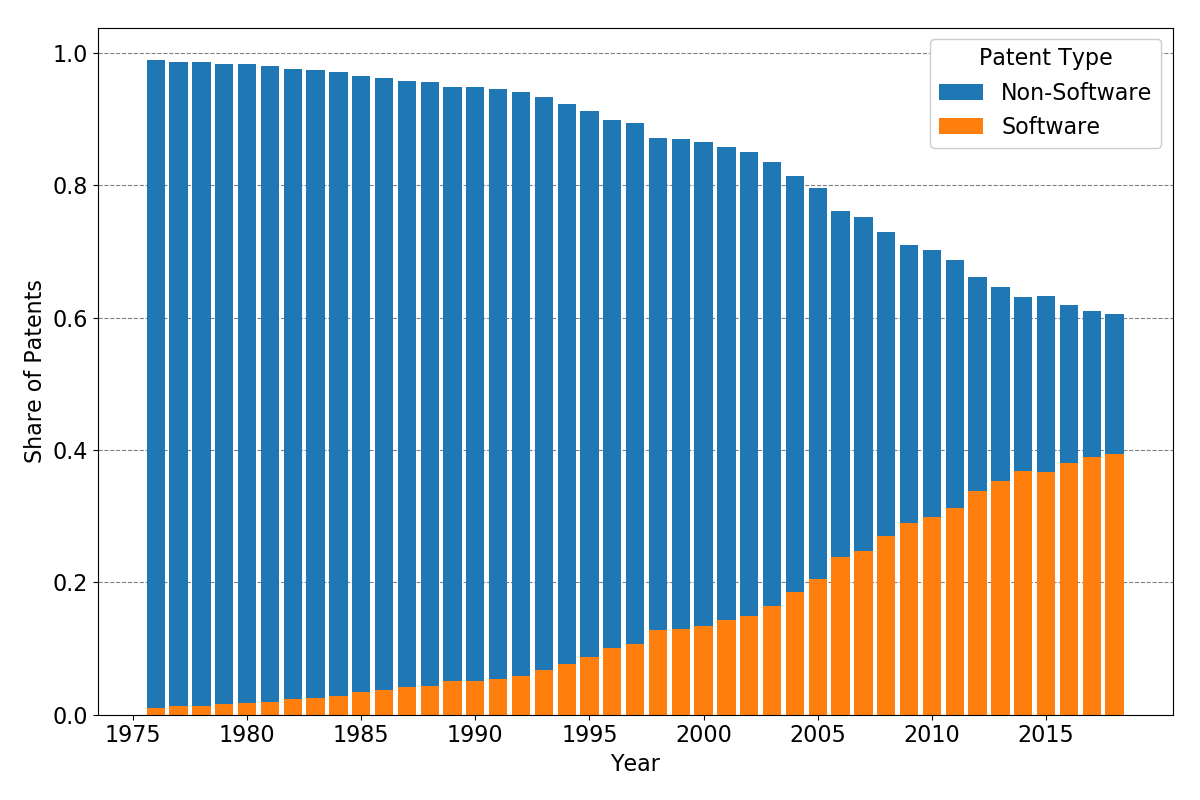
\includegraphics[width=0.7\textwidth]{../../out/figures/fig-patents-distribution-vs-shares}
	\caption{Share of Software Patents}
	\label{fig:sharesoft}
\end{figure}

Furthermore, if the algorithm is applied on all patents from 1976 to 2015, this
results in Figure~\ref{fig:softpat}, which presents the total number of
software patents over the years and Figure~\ref{fig:sharesoft} on the share of
software patents among utility patents. An additional graph is in the appendix:
Figure~\ref{fig:utilpat} on the development of utility patents. The numbers of
utility patents are slowly rising from 65,000 in 1976 to 160,000 in 2010, but
then sharply rising to more than 360,000 in 2014. The numbers of software
patents identified by the algorithm is almost exponentially rising from more
than 10,000 in 1995 to over 150,000 in 2014. The share of software patents on
utility patents is nearly increasing by one percent point each year with a
share of circa 44\% in 2014. Since the developing of software patents is
extreme and might suggest the algorithm is highly overestimating software
patents, other methods to estimate software patents should serve as a
comparison. \citet{graham2013smart} used the experience of Patent Office
experts to identify patent classes and subclasses, which are likely to contain
software patents and used these classes to count software patents. They did not
publish data on software patent counts themselves, but their approach was used
in a report of the Government Accountability Office, which is a U.S. agency
providing auditing, evaluation and investigative services for the United States
Congress. The report\footnote{see \citet{usgao2013}} states the number of
software patents are circa 25,000 in 1991 and about 125,000 in 2011. These
numbers are even higher than the estimates of the algorithm (8,000 in 1991 and
less than 80,000 in 2011). Surprisingly, the algorithm seems to make very
conservative estimations in this comparison. Nonetheless, it is not obvious to
what extent these differences are due to varying definitions.

There are some explanations why there has to be such an increase in software
patents. \citet{bessen2007empirical} point to several court decisions which
reduce the requirements to obtain patent status for software. Another reason
could be the importance of software patents in defensive patenting and as
subject to patent infringement. In this connection it should not be forgotten
that software development is likely to be less capital and resource intensive
than most other technology creation processes. Overly simplified one needs only
knowledge, some hardware, and time.

% subsubsection discussion_of_results (end)
% subsection an_algorithmic_approach (end)

\section{Machine Learning: RandomForestClassifier} % (fold)
\label{sub:machine_learning_randomforestclassifier}

\epigraph{"We are drowning in information and starving for knowledge."}{---
\textup{Rutherford D. Roger}}

This section is about a different approach to identify software patents namely
the application of machine learning techniques. First of all, the broader
context for this approach is explained. After that, random forests are
presented without mathematical detail, but with an intuitive understanding of
the process. At the end, the power of this approach is evaluated.

First of all, what is machine learning about? Machine learning is a subfield of
computer science and related to questions about pattern recognition and
computational learning theory. Prominent applications of machine learning are
spam filters, optical text recognition, and text input recognition on smart
phones. The main difference between computer scientists using machine learning
and statisticians is wrangling with causality. Statistics tries to find
quantitative tools to establish causality in research. In contrast to that,
machine learning practitioners are not concerned about causality. The goal of
their models is to make as accurate predictions as possible.

Giving a short definition, machine learning is the use of algorithms to replace
the pattern recognition process. The advantages of machine learning in contrast
to former methods are automatic rule creation, robustness to errors in
assumptions or modeling, reduced need for explicit programming, and adaption to
changing conditions\footnote{see \cite{kulkarni2011elementary}}.

Machine learning techniques are further divided in several other categories,
but an important distinction for this thesis is supervised and unsupervised
learning\footnote{Other classifications are for example semi-supervised or
reinforcement learning}. Supervised learning is characterized by the fact that
examples are classified with the correct labels whereas unsupervised learning
tries to group the data by itself\footnote{see \cite{kulkarni2011elementary}}.

\begin{figure}[tb]
	\centering
	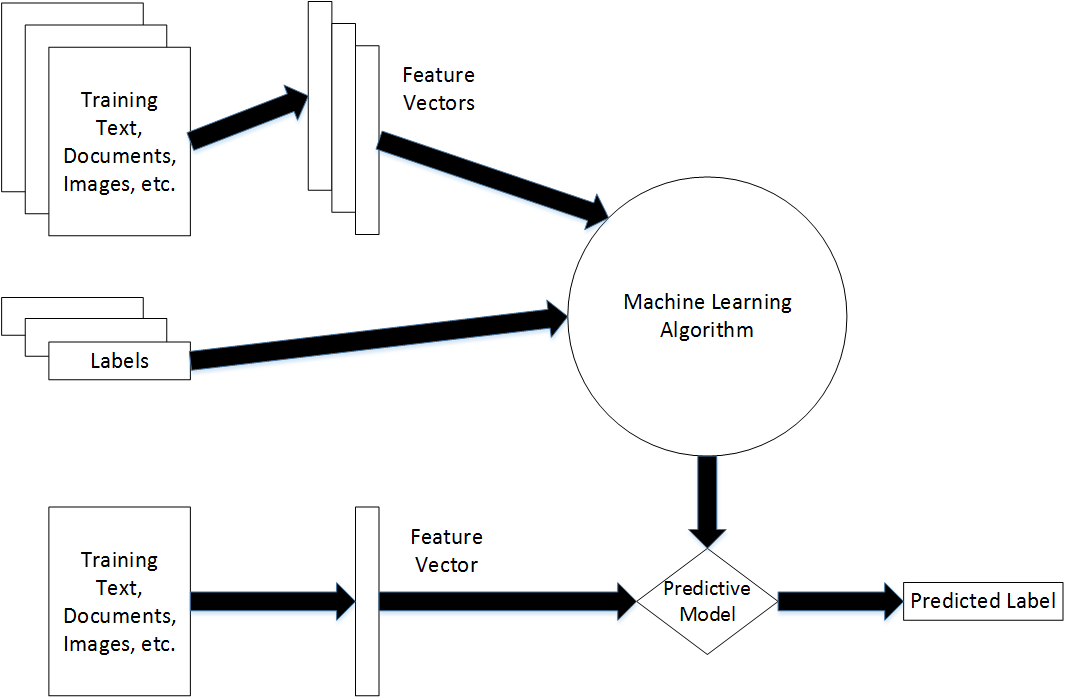
\includegraphics[width = 0.7\textwidth]{graphics/ml_flowchart.png}
	\caption{Flowchart: Supervised learning}
	\label{fig:figure1}
\end{figure}

As the sample of 400 patents of \citeauthor{bessen2007empirical} is already
classified, this analysis focuses on supervised learning. The classification
process starts with labeled data, which means labeled patent texts. While the
labels stay unchanged, the texts are transformed into feature vectors, which
should contain the most valuable information, in processes called feature
extraction and feature selection. The labels and the feature vectors are passed
to the machine learning algorithm which tries to find patterns and rules that
distinguish software and non-software patents. Based on these rules a
predictive model is defined which can assign labels to new patents processed
the same way as the training data.

\subsection{Feature Extraction \& Feature Selection} % (fold)
\label{ssub:feature_extraction_feature_selection}

The tasks of feature extraction and feature selection\footnote{see
\citet[chapter 6]{bird2009natural}} are to take given data as input and
transform it into information which is usable and more informative for the
classifier. Usable means different representations of data are not suitable for
every classifier. The procedure described here is not what represents a common
way to deal with this kind of problem, instead it is a composition of tools
used in the field of NLP with machine learning techniques.

At first, the documents are tokenized, meaning each document is transformed
into an array where the entries represent the sequence of tokens (words,
numbers, and punctuation) in the text ordered by appearance. Then, a vocabulary
matrix is created, which contains the frequency for every different token for
each document\footnote{Another intermediate step which turned out to be not
useful for this analysis is to reduce words to its stem and strip away
suffixes}. Please note, that this matrix contains punctuation, conjunctions,
and other tokens with high frequencies and low variance across the documents
which are not useful for the analysis. They can be deleted by mapping them with
an additional vocabulary or by simply deleting words which occur in ,for
example, 70\%-90\% of all documents. Another problem is that some words only
develop explanatory power considering the context. Therefore, tuples are built
of one token and $n-1$ consecutively tokens. This construction is called n-gram
where $n$ specifies the length of the tuple\footnote{N-grams are also
applicable to the level of letters and yield good results in terms of language
detection}.

The next step involves selecting the most informative features for the
classifier's evaluation process. This step is very important to overcome the
curse of dimensionality\footnote{see \cite{kulkarni2011elementary}}, a
consequence of the imbalance between the number of observations and the
dimension of the feature vector in this sample.
\citeauthor{bessen2007empirical}'s dataset consists of 400 patents, whereas the
vocabulary easily comprises 20,000 different tokens plus the amount of distinct
n-grams in various tuple sizes. If 400 patents populate an approximately
3,000,000 dimensional space, the classifier is likely to rely more on
idiosyncrasies of the sample rather than finding generalized rules. One would
say the classifier is over-fitting.

Firstly, PCA (principal component analysis)\footnote{see
\cite{kuhn2013applied}} is used to identify the most informative features. PCA
tries to find the linear combination of features with the greatest variance to
all data points (patents). This vector is called the first PC. After that, the
subspace which is orthogonal to the first PC is analyzed the same way.
Following this procedure, the whole space is decomposed. The vectors ranked by
the explained variance ratio are passed to the classifier. The goal is to find
hundreds of vectors which cover for example 95\% of the total variance. The
advantage and usefulness of PCA is it creates uncorrelated features which is
important to many classifiers to be numerical stable. But PCA comes along with
two caveats. Because PCA seeks for linear combinations with the maximum
variance, data has to be controlled for skewness, centered and scaled to work
properly. Secondly, PCA is an unsupervised technique and does not take the
label of the data into account. Therefore, if the features' variability is not
related to the label, PCA will not be suitable for the data. This is a serious
problem for the dataset of 400 patents since variance is relatively evenly
distributed among the PCs and not related to software patents deduced from the
results. The approach used in this analysis is the $\chi^2$ statistic, which is
a test to evaluate the independence of two events, label and feature. It
measures how much expected counts deviate from observed counts\footnote{see
\ref{def:chi} for a derivation}. Then, the features with the highest $\chi^2$
statistics are selected for further analysis. Also, one cannot make statements
about the significance level of the features, because the test is used multiple
times and therefore would yield several incorrect tests on average, according
to the significance level. However, if $\chi^2$ is only used to rank the
features and evaluate their relative importance, there should not be any
problems. Nevertheless, this approach is possibly not very useful for this
analysis, because it evaluates only the effect of one feature on the labels. In
that case, features, which are individually not important to software patents,
but powerful in a combination with others are likely to be dropped before the
analysis.

In the next step, the features which have been extracted and selected, are
passed to the classifier, which will deduce rules from the information
connected to the labels. The classifier is explained in the following section.

\subsection{The Random Forest Classifier} % (fold)
\label{sub:the_random_forest_classifier}

\begin{figure}[tb]
	\centering
	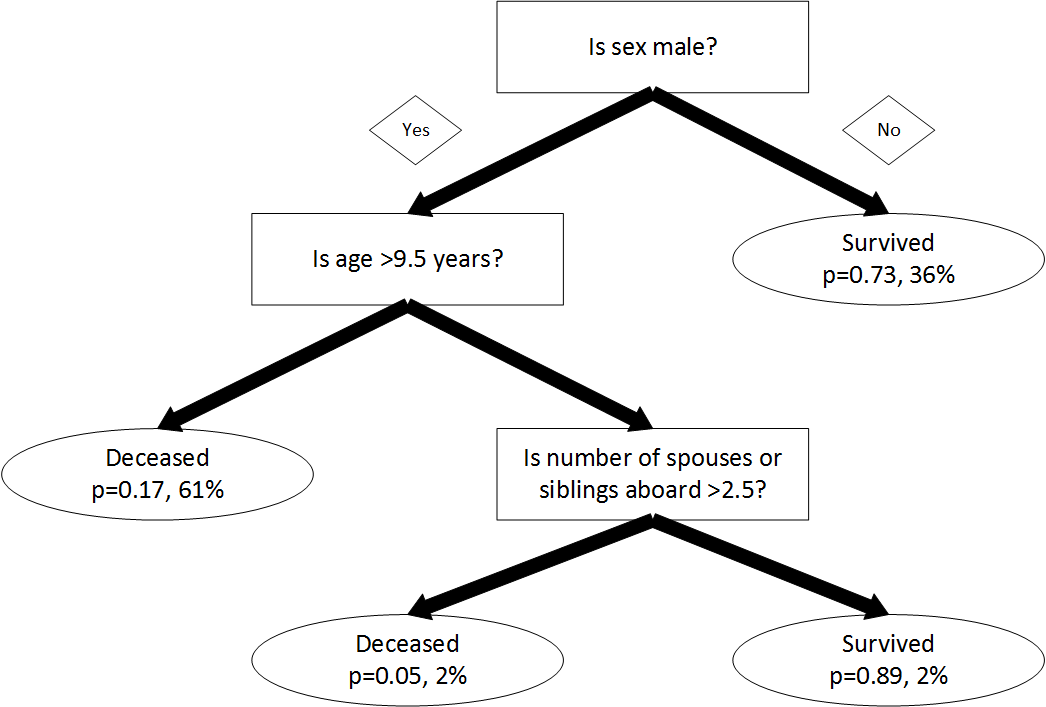
\includegraphics[width=0.7\textwidth]{graphics/titanic.png}
    \caption{This is an example of an decision tree predicting survival rates
    of passengers of the RMS Titanic. The numbers below the prediction are the
    probability of survival and the percentage of observations of the sample}
	\label{fig:decisiontree}
\end{figure}

The machine learning approach to classify software patents will use random
forests, member of a bigger group of machine learning classifiers called
ensemble learning. The key aspect of these methods is to build a prediction
model which is based on a collection of simpler base models\footnote{see
\citet[Chapter 16]{friedman2009elements}}. In this case, random forests average
over the prediction of many decision trees and therefore perform better than an
individual decision tree. The idea behind decision trees is that beginning at a
parent node, they partition the feature space according to a splitting rule and
by that creating new nodes with subsets of the data. The splitting rule is
repeatedly applied until a certain limit. The last nodes in the tree do not
separate the sample any further, instead they have leaves attached to them,
which contain the prediction. An example of a decision tree with data on the
sinking of the RMS Titanic is show in Figure~\ref{fig:decisiontree}.

\begin{figure}[!ht]
	\centering
	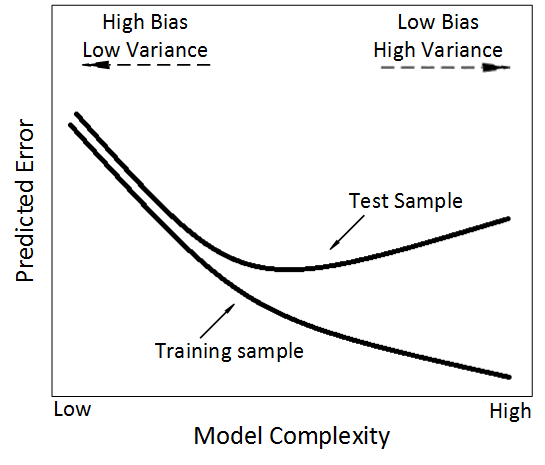
\includegraphics[width=0.7\textwidth]{graphics/biasvariancetradeoff.png}
	\caption{Bias-Variance-Trade-off}
	\label{fig:biasvariancetradeoff}
\end{figure}

The power of random forests lies in the bias-variance-trade-off\footnote{see
\citet[Chapter 2]{friedman2009elements}} which is determined by the models
complexity and the prediction error. Figure~\ref{fig:biasvariancetradeoff}
shows, the prediction error of the training sample decreases with rising
complexity. The model gets better in fitting the data up to the point of
virtually no prediction error, when it is simply memorizing the training data.
The curve for the test sample is first decreasing and then increasing in the
model's complexity. On the left side of its minimum the model has not
generalized enough and is therefore biased, called underfitting. In contrast to
that, on the right side the model is overfitting, because it focuses more on
idiosyncrasies of the training sample than on generalization.

% Boosting, introduced by \cite{freund1999short}, is the first concept to
% exploit the trade-off. High bias but low variance models, such as not
% sufficiently deep grown decision trees, are called weak learners. They
% perform slightly better than pure random, which can be used to establish a
% strong learner. Weak learners are fitted on repeatedly modified versions the
% data. When they are added to a strong classifier, they are weighted in
% relation to their former accuracy. After that, the data is reweighted, so
% that previous misclassified examples in the data gain more weight than the
% correct classified data. Therefore, following weak learners are forced to
% concentrate on the errors of previous learners.

Bagging\footnote{see \cite{breiman1996bagging}} was invented to overcome this
trade-off to some extent. The idea behind this is similar to the observation of
$Z_1, Z_2, \dots, Z_n$ independent variables with variance $\sigma^2$, whereas
the mean $\bar{Z}$ has a variance $\frac{\sigma^2}{n}$. So, a set of
observations is averaged to reduce the variance, which is normally not
practical, because there is only one training set. Therefore, bagging creates
many samples by randomly drawing observations from the training set with
replacement until the number of observations is equal to the original sample.
This kind of sample generation is called bootstrapping. But unlike the example
with the independent $Z_i$ variables the predictions $T_b(x)$ of a tree $b$
with the features $x$ are not independent, since the samples are all drawn from
the same population. This can also be presented by the variance of the whole
forest\footnote{see \ref{def:bootstrap} for a derivation}:

\begin{align*}
Var(\frac{1}{B}\sum^B_{b = 1} T_b(x)) = \rho\sigma^2 + \frac{1-\rho}{B}\sigma^2
\end{align*}

The second term diminishes with a higher number of trees $B$, but the first
term can only be decreased by reducing the correlation $\rho$ among the trees.
That is why, randomness has to be induced into the model. Hence, only a random
share of all variables in the sample is considered at each split during the
tree-growing process. According to \cite{friedman2009elements}, the square root
of the number of features is a default number for features considered at each
split, whereas in this analysis only a third of all observations is used.
Because the split is no longer the best split among all variables, the bias of
the decision tree slightly increases, but it is normally more than compensated
by the decrease in variance\footnote{Better reference than scikit-learn}.

To recap, the randomness increases as the number of features considered at each
split is lowered. Therefore, the variance of the average over all predictions
is lowered and the results are more precise. This is all due to a concept
called bagging in which many decision trees are grown on bootstrap samples.

\begin{table}[!ht]
	\caption{Random Forest for Classification \citep{friedman2009elements}}
	\label{tab:randomforest}
	\centering\ra{1.3}
	\begin{tabular}{@{}llll@{}}\toprule
	1.	& \multicolumn{3}{l}{For $b=1$ to $B$:}\\
		& (a) & \multicolumn{2}{p{13cm}}{Draw a bootstrap sample \textbf{Z}* of size N from the training data.}\\
		& (b) & \multicolumn{2}{p{13cm}}{Grow a random-forest tree $T_b$ to the bootstrapped data, by recursively repeating the following steps for each terminal node of the tree, until the minimum node size $n_{min}$ is reached.}\\
		& & i. & Select $m$ variables at random from the $p$ variables.\\
		& & ii. & Pick the best variable/split-point among the $m$.\\
		& & iii. & Split the node into two daughter nodes.\\
	2.	& \multicolumn{3}{l}{Output the ensemble of trees $\{T_b\}^B_1$.}\\[0.25cm]\midrule
	\multicolumn{4}{l}{To make a prediction at a new point $x$:}\\
	\multicolumn{4}{p{15cm}}{\textit{Classification}: Let $\hat{C}_b(x)$ be the class prediction of the $b$th random-forest tree. Then $\hat{C}^B_{rf}(x) = majority\ vote\ \{\hat{C}_b(x)\}^B_1$.}\\
	\bottomrule
	\end{tabular}
\end{table}

The splitting rule choosing the most informative variable at a given node has
to be defined. There are many metrics to choose the variable like variance
reduction and information gain, which is based on entropy from information
theory. The criterion used in this analysis is the Gini index\footnote{see
\citet[Chapter 9.2]{friedman2009elements} and
\citet{breiman1984classification}}, or, better, Gini impurity which should not
be confused with the Gini coefficient, a measure of inequality. If subsets with
Gini impurity are constructed, then one has maximized the homogeneity of the
child nodes depending on the parent node over all features and all of its
values. The formula to compute the Gini impurity in a given node $t$, when the
split is made on one feature value, is:

\begin{align*}
I_G(t) = \sum_{k\neq l}p(k|t)p(l|t) \overset{\text{two classes}}{=} 2\cdot p(1|t)p(2|t) = 2\cdot p(1|t)(1-p(1|t))
\end{align*}

$k$ and $l$ are indices for the classes and $p(k|t)$ is the conditional
probability of class $k$ in node $t$\footnote{A more detailed look on this
problem is presented in \ref{def:giniimpurity}}.

Another remark concerns one difference between the prediction model used here
and the standard model in Table~\ref{tab:randomforest}, which assigns labels
following the majority of votes generated by each tree. The random forest in
this analysis uses predicted class probabilities. They are calculated as the
mean predicted class probabilities of the trees in the forest. The class
probability of a single tree is the fraction of samples of the same class in a
leaf.

% subsection the_random_forest_classifier (end)

\subsection{Results} % (fold)
\label{sub:results}

The results of the prediction are calculated using cross-validation, which is
statistic tool to evaluate the performance of a predictive model on an
independent dataset. Hence, it iteratively separates the data into a training
sample and a test sample randomly drawn without replacement and pass both to
the classifier. The results of the classifier depending on the different
compositions can be averaged and the overall score serves as an approximation
to result on independent data. This procedure should prevent overfitting of the
classifier during the tuning process and limit the error of testing hypothesis
suggested by the data, which refers to the problem of drawing conclusions from
a limited dataset and then confirm the results by using the same. The exact
method used in this thesis is a 10-fold-stratified-cross-validation, which
means 10 training and 10 test samples are created to evaluate the performance.
Furthermore, the term stratified indicates that the subsamples have the same
ratio of software and non-software patents as the original sample. This is
necessary, because of the skewness of the data and to prevent imbalances.

Another point has to be made about the separation of the data. The normal
scientific procedure would be to divide the available classified data in a
training set and a test set. Then, the training set is further divided into
train and test samples by cross-validation to tune the classifier. At last, the
classifier is applied on the unseen test sample and results are reported, which
are a better indicator for performance on new data. Due to the lack of
classified patents, the data could not be further divided and therefore the
reported results are from cross-validation. One would suggest that the results
are overly optimistic.

\begin{table}[tb]\caption{The confusion matrix shows the aggregated counts for
each field of a 10-fold-stratified-cross-validation using 10\% of the data for
testing}\label{tab:confusion_ml_results}\centering\ra{1.3}
\begin{tabular}{@{}cp{0.5cm}cp{0.5cm}c@{}} \toprule
 & & Relevant & & Not Relevant\\ \cline{1-1} \cline{3-3} \cline{5-5}
Retrieved & & 36 & & 8\\
Not Retrieved & & 14 & & 342\\
\bottomrule
\end{tabular}
\end{table}

The aggregated results suggest that the random forest classifier performs not
as good on the sample as the algorithm by \citet{bessen2007empirical}. The
$\kappa$ for the algorithm was 78\%, whereas the value for the classifier is
73\%\footnote{see Table~\ref{tab:eval_machine_learning} for more metrics}. The
main reason for that can be seen by observing the $\kappa$ statistic for each
of the 10 folds. The $\kappa$ is ranging from 31\% to 89\%\footnote{All
$\kappa$ values for each fold are presented in
Table~\ref{tab:kappastatistics}}, which indicates that the composition of the
samples is highly influencing the results. That means, 399 patents are not
enough data to train the algorithm properly and to identify really generalized
rules for the distinction between software and other patents\footnote{Due to
time constraints, the sample could not be extended for further analysis.}.

Considering the structure of both approaches, it is obvious that the algorithm
only establishes a lower bound for the random forest classifier. A linear
combination of keywords such as the algorithm is easily captured by the
decision trees. Furthermore, random forests can rely on much richer vocabulary
and differentiate between occurrences and frequencies.

Taken all together, this approach is one example to deal with the topic of
patent identification using tools from machine learning. Although, the results
were not as good as the previous algorithm, the work with machine learning
techniques should prove to be more fruitful using more domain expertise on both
patents and machine learning.

% subsection results (end)
% section identification_strategies (end)

\section{Conclusion} % (fold)
\label{sec:results}

In the first part of the thesis, the need for identification strategies for
patents is described. It started with an overview of patents, the structure of
the data and a discussion on patents' quality as an indicator for technological
progress. After that, two studies are presented with applications of two
different identification strategies. The second part explores two different
approaches, an algorithm which identifies patents by word occurrences and a
random forest classifier which derives a generalization of a software patent
from a training set based on token frequencies. In the end the second strategy
is not comparable to the first since the sample size  caused unstable
predictions during cross-validation. Furthermore, the idea to use machine
learning techniques to extend this thesis came up during the writing process.
After one month wrangling with those techniques, this thesis represents the
first steps into the field of machine learning.

% section results (end)

\newpage

\appendix
\section*{Appendices}
\addcontentsline{toc}{section}{Appendices}
\renewcommand{\thesubsection}{\Alph{subsection}}

\subsection{Tables}

\begin{table}[!hp]\caption{Confusion Matrix Example}\label{tab:confusion_example}\centering\ra{1.3}
\begin{tabular}{@{}cp{0.5cm}cp{0.5cm}c@{}} \toprule
 & & Relevant & & Not Relevant\\ \cline{1-1} \cline{3-3} \cline{5-5}
Retrieved & & true positives (tp) & & false positives (fp)\\
Not Retrieved & & false negatives (fn) & & true negatives (tn)\\
\bottomrule
\end{tabular}
\end{table}

\begin{table}[!hp]\caption{Definitions of Measures}\label{tab:definition_measure}\centering\ra{2}
\begin{tabular}{@{}cp{2cm}c@{}} \toprule
Measure & & Definition\\ \cline{1-1} \cline{3-3}
Accuracy & & $\frac{tp + tn}{tp + fp + fn + tn}$\\
Precision & & $\frac{tp}{tp + fp}$\\
Recall & & $\frac{tp}{tp + fn}$\\
Expected Accuracy & & $\sum^n_{i=1}\sum^n_{j=1}\frac{h_{\cdot j}}{n}\cdot\frac{h_{i \cdot}}{n}$\\
$\kappa$ & & $\frac{\text{Accuracy} - \text{Expected Accuracy}}{1 - \text{Expected Accuracy}}$\\
\bottomrule
\end{tabular}
\end{table}

\begin{table}[!hp]\caption{Evaluation table of \cite{bessen2007empirical}}\label{tab:eval_algo_original}\centering\ra{1.3}
\begin{tabular}{@{}cp{0.5cm}cp{0.5cm}cp{0.5cm}cp{0.5cm}c@{}} \toprule
 & & Precision & & Recall & & $\kappa$ & & Support\\ \cline{1-1} \cline{3-3} \cline{5-5} \cline{7-7} \cline{9-9}
non-software & & 0.97 & & 0.98 & &  & & 345\\
software & & 0.84 & & 0.78 & &  & & 54\\ \cline{1-1} \cline{3-3} \cline{5-5} \cline{7-7} \cline{9-9}
avg / total & & 0.95 & & 0.95 & & 0.78 & & 399\\
\bottomrule
\end{tabular}
\end{table}

\begin{table}[!hp]\caption{Evaluation table of replication}\label{tab:eval_algo_rep}\centering\ra{1.3}
\begin{tabular}{@{}cp{0.5cm}cp{0.5cm}cp{0.5cm}cp{0.5cm}c@{}} \toprule
 & & Precision & & Recall & & $\kappa$ & & Support\\ \cline{1-1} \cline{3-3} \cline{5-5} \cline{7-7} \cline{9-9}
non-software & & 0.97 & & 0.95 & &  & & 345\\
software & & 0.71 & & 0.83 & &  & & 54\\ \cline{1-1} \cline{3-3} \cline{5-5} \cline{7-7} \cline{9-9}
avg / total & & 0.94 & & 0.93 & & 0.72 & & 399\\
\bottomrule
\end{tabular}
\end{table}

\newpage

\begin{table}[!hp]\caption{Evaluation table of replication}\label{tab:eval_machine_learning}\centering\ra{1.3}
\begin{tabular}{@{}cp{0.5cm}cp{0.5cm}cp{0.5cm}cp{0.5cm}c@{}} \toprule
 & & Precision & & Recall & & $\kappa$ & & Support\\ \cline{1-1} \cline{3-3} \cline{5-5} \cline{7-7} \cline{9-9}
non-software & & 0.96 & & 0.97 & &  & & 350\\
software & & 0.81 & & 0.72 & &  & & 50\\ \cline{1-1} \cline{3-3} \cline{5-5} \cline{7-7} \cline{9-9}
avg / total & & 0.94 & & 0.93 & & 0.73 & & 400\\
\bottomrule
\end{tabular}
\end{table}

\begin{table}[!hp]\caption{$\kappa$ statistics for each of the 10-fold-stratified-cross-validation}\label{tab:kappastatistics}\centering\ra{1.3}
\begin{tabular}{cp{1mm}cp{1cm}cp{1mm}c} \toprule
\# & & $\kappa$ & & \# & & $\kappa$\\ \cline{1-1} \cline{3-3} \cline{5-5} \cline{7-7}
1 & & 0.875 & & 6 & & 0.875 \\
2 & & 0.875 & & 7 & & 0.543 \\
3 & & 0.875 & & 8 & & 0.875 \\
4 & & 0.771 & & 9 & & 0.448 \\
5 & & 0.895 & & 10 & & 0.314 \\
\bottomrule
\end{tabular}
\end{table}

\begin{table}[!hp]\caption{List of Urls}\label{tab:url}\centering\ra{1.3}
\begin{tabular}{cp{0.5cm}p{5cm}p{0.5cm}p{5cm}}\toprule
\# & & Description & & Url\\ \cline{1-1} \cline{3-3} \cline{5-5}
1 & & US Patent Statistic Chart with numbers of patent applications and grants from 1963 to 2015 & & \url{http://goo.gl/fK6Upx}\\
2 & & European Patent Office Application statistics & & \url{http://goo.gl/ncsWqf}\\
3 & & European Patent Office Grants statistics & & \url{http://goo.gl/bL44zq}\\
4 & & The NBER U.S. Patent Citations Data File & & \url{http://www.nber.org/patents/}\\
5 & & Nokia suing Apple in October 2009 & & \url{http://goo.gl/99uZoW}\\
6 & & Apple suing Nokia in December 2009 & & \url{http://goo.gl/Iewdih}\\
7 & & USPTO list of withdrawn patents & & \url{http://goo.gl/iLjInp}\\
8 & & Explanation: Withdrawal from Issue & & \url{http://goo.gl/GgI9yN}\\
9 & & John Oliver's report on patents & & \url{https://youtu.be/3bxcc3SM_KA}\\
\bottomrule
\end{tabular}
\end{table}




\newpage

\subsection{Graphics}

\begin{figure}[!ht]
	\centering
	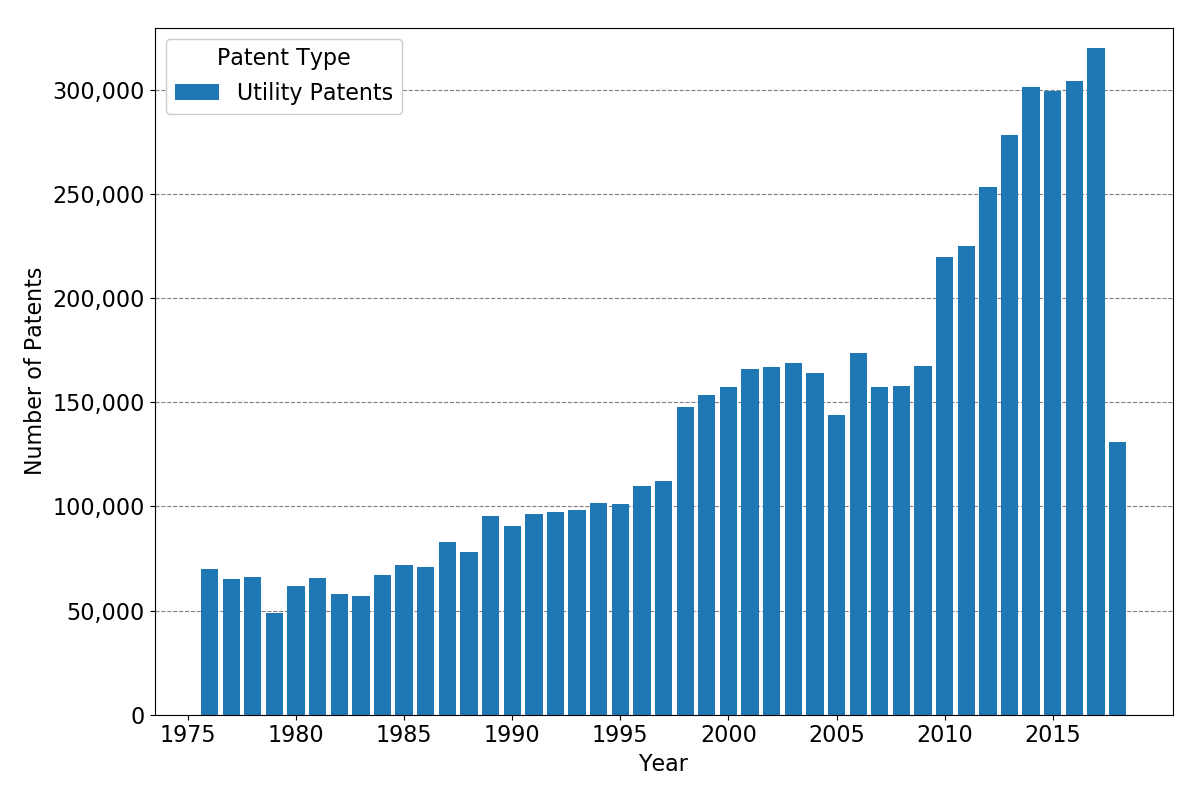
\includegraphics[width=0.9\textwidth]{../../out/figures/fig-patents-distribution}
	\caption{Number of Utility Patents}
	\label{fig:utilpat}
\end{figure}

\newpage

\subsection{Definitions, Data, et cetera}

\begin{definition}The algorithm is defined as\footnote{\citet[p.29]{bessen2007empirical}}:
\label{def:algo}

\bigskip
\texttt{
\begin{tabular}{p{3cm}p{10cm}}
 & (("software" in specification) OR ("computer" AND "program" in specification))\\
AND & (utility patent excluding reissues)\\
ANDNOT & ("chip" OR "semiconductor" OR "bus" OR "circuit" OR "circuitry" in title)\\
ANDNOT & ("antigen" OR "antigenic" OR "chromatography" in specification)
\end{tabular}
}\bigskip

Specification refers to the abstract plus the description of the patent.
\end{definition}\vspace{2cm}

\begin{definition}The $\chi^2$ statistic for one feature and one label is\footnote{\cite{manning2008introduction}}:
\label{def:chi}

\bigskip

\begin{align*}
&\chi^2 = \sum^r_{i = 1}\sum^c_{j = 1}\frac{(O_{i,j}-E_{i,j})^2}{E_{i,j}} & &\\
\text{with } &O_i  &\text{, as observations of type i}\\
\text{with } &E_{i,j} = Np_ip_j &\text{, as expected observations}\\
\text{with } &p_{i\cdot} = \sum^c_{j = 1}\frac{O_{i,j}}{N} &\text{, as the average of observation i}\\
\text{with } &p_{\cdot j} = \sum^c_{i = 1}\frac{O_{i,j}}{N} &\text{, as the average of observation j}\\
\end{align*}
\end{definition}\vspace{6cm}

\begin{definition}
The variance of multiple decision trees grown on bootstrap samples is derived
here\footnote{see \cite{friedman2009elements}}:

\begin{align*}
Var(\frac{1}{B}\sum^B_{i=1}T_i(x)) &= \frac{1}{B^2}\sum^B_{i=1}\sum^B_{j=1}Cov(T_i(x), T_j(x))\\
&= \frac{1}{B^2}\sum^B_{i=1}(\sum^B_{j\neq i}Cov(T_i(x), T_j(x)) + Var(T_i(x)))\\
&= \frac{1}{B^2}\sum^B_{i=1} ((B-1)\sigma^2\rho + \sigma^2)\\
&= \frac{B(B-1)\rho\sigma^2 + B\sigma^2}{B^2}\\
&= \frac{(B-1)\rho\sigma^2}{B} + \frac{\sigma^2}{B}\\
&= \underbrace{\rho\sigma^2}_{\text{decreases with de-correlation}} + \underbrace{\sigma^2 \frac{1-\rho}{B}}_{\text{decreases in number of trees}}
\end{align*}
\label{def:bootstrap}
\end{definition}\vspace{2cm}

\begin{definition}
This is the derivation of the problem, which is solved at each split in a
decision tree\footnote{see \citet{breiman1984classification}}:

Consider $t_p$ as a parent node and $t_l$ and $t_r$ the child nodes to the left
and right. A training dataset $X$ is given with $M$ features and $N$
observations. There is also a label vector $Y$ with $N$ observations and $K$
classes.

\begin{figure}[!ht]
	\centering
	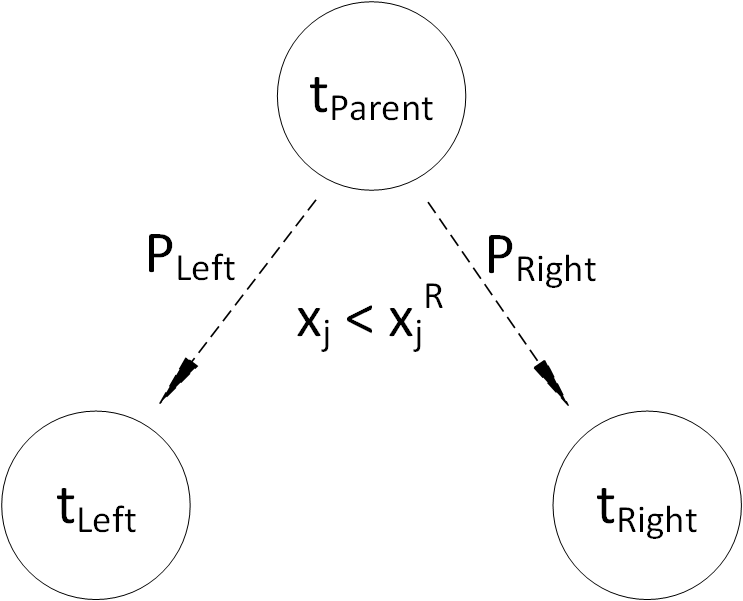
\includegraphics[width=0.5\textwidth]{graphics/giniimpurity.png}
	\caption{Decision Tree Example with split at $x^R_j$}
	\label{fig:giniimpurity}
\end{figure}

The split in this example is done by variable $x^B_j$, which is the best split
among values of variable $x_j$. The goal is to establish the maximum
homogeneity among the results, which is defined by an impurity function $i(t)$.
The impurity gain of a split can be defined as:

\begin{align*}
\delta i(t) = i(t_p) - E[i(t_c)]
\end{align*}

The impurity among the child nodes $t_c$ is weighted by numbers of observation
in the sample. This probability is defined as $P_l$ and $P_r$.

\begin{align*}
\delta i(t) = i(t_p) - P_li(t_l) - P_ri(t_r)
\end{align*}

This example can be generalized to a maximization problem over all variables
and values to find the split with the highest impurity gain.

\begin{align*}
\underset{x_j\leq x^R_j,j=1,\dots,M}{\arg\max}\hspace{5mm} i(t_p) - P_li(t_l) -P_ri(t_r)
\end{align*}

Now, let the impurity function be Gini impurity, which is defined as the
following with $k\in[1,\dots,K]$ as the index of the class and $p(k|t)$ as the
conditional probability of class $k$ in node $t$:

\begin{align*}
i(t) = \sum_{k\neq l} p(k|t) p(l|t) = 1-\sum_kp^2(k|t)
\end{align*}

Inserting this function into the formula for $\delta i(t)$ it yields:

\begin{align*}
\delta i(t) = -\sum^K_{k=1}p^2(k|t_p) + P_l\sum^K_{k=1}p^2(k|t_l) + P_r\sum^K_{k=1}p^2(k|t_r)
\end{align*}

And for the maximization problem:

\begin{align*}
\underset{x_j\leq x^R_j,j=1,\dots,M}{\arg\max}\hspace{5mm} -\sum^K_{k=1}p^2(k|t_p) + P_l\sum^K_{k=1}p^2(k|t_l) + P_r\sum^K_{k=1}p^2(k|t_r)
\end{align*}
\label{def:giniimpurity}
\end{definition}

\newpage

\printbibliography

\newpage

\vspace*{5cm}

\textbf{\Large Schriftliche Versicherung}\vspace{3cm}

„Ich versichere hiermit, dass ich die vorstehende Bachelorarbeit selbstständig
verfasst und keine anderen als die angegebenen Quellen und Hilfsmittel benutzt
habe, dass die vorgelegte Arbeit noch an keiner anderen Hochschule zur Prüfung
vorgelegt wurde und dass sie weder ganz noch in Teilen bereits veröffentlicht
wurde. Wörtliche Zitate und Stellen, die anderen Werken dem Sinn nach entnommen
sind, habe ich in jedem einzelnen Fall kenntlich gemacht.“

\vspace{3cm}

\begin{tabular}{p{4cm}p{4cm}p{4cm}} \\
&  & \\ \cline{1-1} \cline{3-3}
\footnotesize{Ort, Datum} & & \footnotesize{Unterschrift}\\
\end{tabular}

\end{document}